\documentclass{article}

\usepackage[margin=1in]{geometry}
\usepackage{amsmath,amssymb, bbm}
\usepackage[backend=biber,
	style=alphabetic,
	%	citestyle=authoryear,
	natbib=true,
	url=true, 
	doi=true]{biblatex}

\addbibresource{../refs.bib}
\addbibresource{../maths.bib}

\usepackage{microtype}
\usepackage{relsize}
\usepackage{tikz}
	\usetikzlibrary{positioning,fit,calc, arrows, shapes}
	
	\tikzset{dpadded/.style={rounded corners=2, inner sep=1em, draw, outer sep=0.5em}}
	\tikzset{active/.style={fill=blue, fill opacity=0.1, text opacity=1}}

	\tikzset{pt/.style args={#1}{name=#1, circle, fill, inner sep=1pt,label={[name={lab-#1},gray]\scriptsize #1}} }
	\tikzset{mpt/.style args={#1|#2}{name=#1, circle, fill, inner sep=1pt,label={[name={lab-#1},gray]\scriptsize #2}} }
		
		 %\foreach \x in {#1}{(\x) (lab-\x) } 
	\tikzset{Dom/.style args={#1 : #2}{dpadded, name=#1, label={[name={lab-#1}] #1}, fit={ #2 } }}
	\tikzset{bDom/.style args={#1 : #2}{dpadded, name=#1, label={[name={lab-#1}]below:#1},  fit={ #2 } }}
	\tikzset{arr/.style={->, thick, shorten <=3pt, shorten >=3pt}}
	%\tikzset{every label/.append style={text=red, font=\scriptsize}}

\usepackage{color}
\definecolor{deepgreen}{rgb}{0,0.5,0}

\usepackage[colorlinks=true, citecolor=deepgreen]{hyperref}


\setlength{\skip\footins}{1cm}
\setlength{\footnotesep}{0.4cm}

\usepackage{parskip}
\usepackage{amsthm}
\begingroup
\makeatletter
\@for\theoremstyle:=definition,remark,plain\do{%
	\expandafter\g@addto@macro\csname th@\theoremstyle\endcsname{%
		\addtolength\thm@preskip\parskip
	}%
}
\endgroup

\theoremstyle{plain}
\newtheorem{theorem}{Theorem}[section]
\newtheorem{coro}{Corollary}[theorem]
\newtheorem{prop}[theorem]{Proposition}
\newtheorem{lemma}[theorem]{Lemma}
\newtheorem{fact}[theorem]{Fact}
\newtheorem{conj}[theorem]{Conjecture}

\theoremstyle{definition}
\newtheorem{defn}{Definition}[section]
\newtheorem{example}{Example}[section]

\theoremstyle{remark}
\newtheorem*{remark}{Remark}


\usepackage{enumitem}


%\newcommand\duplicat[1]{\gdef\mylist{}\foreach \x in {#1}{\xdef\mylist{\mylist (\x) (lab-\x) }}\mylist} %% this doesn't work :((
\newcommand\lab[1]{(#1)(lab-#1)}


\newcommand{\todo}[1]{{\color{red}\large\textbf{[todo}: {\normalsize\itshape#1}\textbf{]}}}
\newcommand\geqc{\succcurlyeq}
\newcommand\leqc{\preccurlyeq}
\newcommand\mat[1]{\mathbf #1}
\newcommand{\indi}[1]{\mathbbm{1}_{\left[\vphantom{\big[}#1 \vphantom{\big]}\right]}}

\title{A Theory of Dynamic Preferences}
\author{Oliver Richardson  \texttt{oli@cs.cornell.edu}}

\begin{document}
	\maketitle
	\section{A Broad Picture of Decision Making}
	If you already have a (A) model of the world which is detailed enough to describe all possible things that can happen, and in addition you have both (B) beliefs about how the world is likely to evolve in response to any of your actions, and (C) preferences over all possible sequences of events that could happen, then classical decision theories such as Savage's \cite{savage1972foundations} or Jeffrey's \cite{jeffrey1990logic} gives satisfying answers to (D) decision problems  --- at least, given enough computational power.
	
	Unfortunately, all three of these components are difficult to get. A perfect world representation (A) seems impossible, but by providing models at a higher abstraction, we can bypass this and proceed with the caveat that decisions can only be as good as the model. Given (A) and some not entirely broken guess at (B), Bayesian updating tells you how to iteratively refine (B) from observations. Representation learning provides some answers about how to refine (A) and (B) at the same time if you already have a task (C) in mind. Model-free reinforcement learning skips the decision theory bit entirely, and uses a reward function (C) to infer actions (D) directly, implicitly refining both (A) and (B) based on experiences.
		
	The work done in search of acquiring preferences (C) preferences has been much less thorough, in part because preferences have always been the grounding used to evaluate the other components of the decision making process. However with so many advances in the other areas of decision making, acquiring the right preferences has recently become a bottleneck, and extremely important: 
	
	\begin{itemize}[]
		\item Recommender systems, such as the YouTube sidebar, targeted advertising, internet radio, and even search algorithms, have the job of learning users' preferences (both individual and collective) about content. This makes good models of preference dynamics useful directly for predictive power in humans.
		
		\item These learning systems and others have objective functions which they optimize---preferences of their own---but getting these objective functions ``wrong'' can result in systems that are totally useless, such as game playing agents that incur no loss by pausing the game, ad delivery systems that plaster the page in ads to maximize ad clicks. Worse, they can appear right at first, but have nasty side effects: unfairly reinforcing inequality, serving news that reinforces confirmation biases, and so forth.
		
		\item Both markets and democracies can also be thought of as optimization procedures for specific objectives (defined by the currency and voting systems, respectively). Both have well-documented failure cases, and in response, many have come up with alternative ways of regulating trade and counting votes. But how do we determine if they're any good? We would need a model of preference updates.
		
		\item  Many now worry that an artificial general intelligence (AGI), smart enough to out-maneuver humanity, but with undesirable preferences (``unaligned'') is becoming increasingly likely. Many serious AI practitioners take this concern seriously: DeepMind, OpenAI, MIRI, and FHI all have AI safety divisions for this reason. OpenAI and Google Brain's seminal paper \cite{amodei2016concrete} details many of the particular concerns and the current ideas we have for solving them.
		
	\end{itemize}

	I think it is important to mention that, while these are all issues that have only recently become problematic, the general problem of having to figure out what to care about has been a (and arguably the only) fundamental problem in philosophy for a long time: ethics is a field dedicated to deciding what we should care about; meta-ethics a field about how to make those decisions. Sociological accounts of cultural revolution and art history both are also both theories of preference change in specific domains.
	
	%More indirectly, philosophy of physics can be thought of as a clarification of what physicists should care about, etc.
	
	Even the specific worries about mis-specifying objectives to powerful optimizing procedures have ancient cultural roots: there are endless stories and jokes of leprechauns, genies, and monkey paws granting wishes that turned out to have unintended side effects. 
	
	This is all to say: the problem at hand is enormously important, and people have already put an enormous of work into it. And yet, none of few formal theories of preference acquisition and updating has received much attention, and none of them are in dialog with ML theory. It is crazy to expect that the single contribution I make here could single-handedly render all of this other work obsolete, but it is rather intended that this will provide a unified language and formalism that others can use to represent their own models and solutions, some general results which could be used as support for positions in any of these fields, and also some that are more specific to the setting of machine preference updates.
		
	\subsection*{Responses to some preliminary concerns}
	Nobody doubts that getting the ``right'' preferences are important, but there are a number of reasons that people might see this as a garbage research agenda; before continuing, I'd like to quickly address a few of these:
	
	\textbf{There's no such thing as ``right''.} The first issue has to do with the quotation marks that I've put around the morally loaded words I've used up until now. Moral relativism, perhaps in combination with an intuition of preferences that comes from classical economic theory, would suggest that every preference is equally valid. This viewpoint also meshes well with the distinction emotion / reason dichotomy people like to draw, and the orthogonality thesis \cite{bostrom2012superintelligent}. In this view, the merit of something can only be evaluated with respect to your own preferences, and \todo{preference updating merits}
	
%	That's just like, your 
	
	
	\textbf{This all just boils down to one more objective you've put on top.} \todo{implicit objective may be better, if it has desirable properties}
	


	\subsection*{Relevant Work in Representing, Acquiring, and Updating Preferences}
	
	 %The so-called Gandhi-Folk theorem 
	
	Bayesian Networks are a particularly relevant technique for representing (2), and represent a factorization of a joint probability distribution across a number of variables $N$ as the product of conditional probability distributions associated with the edges of a graph whose nodes are $N$.	
	
	

	 CP Nets \cite{boutilier2004cp} are one attempt to factor preferences analogously to Bayesian Networks, but they suffer from a number of issues, which we will explore in section \ref{sec:bad-cpnets}. 
	
	
	Drawing the analogy further, observations 	
	
	\todo{finish background: Inverse Reinforcement Learning, CP Nets, Girard, Fenrong, Skill Babling, Policy Space Topology, Taxonomy from 2009 Pref Change book}
	
%	\subsection*{A Broad Intuition For This Theory}
	
	
	\section{What I want to do}
	I'm trying to get a theory of preference dynamics.
	
	Currently preferences are thought of as static objects, fixed as part of the structure and identity of an agent, independent of beliefs, complete, and over some fixed domain. This is clearly not at all how human preferences work, and I posit that it's not the right way to think of preference for synthetic agents either.
	
	Perhaps among other things, desiderata for a model of preference dynamics should:
	\begin{enumerate}[noitemsep]
		\item Provide an answer to the `value loading' problem: show how you can acquire ``reasonable'' preferences by interacting with the world
		\item Reduce to static models for some parameter settings
		\item Behave reasonably when combined with changes of perspective 
		\item Be resistant to standard challenges to irrationality, such as dutch booking
		\item Have weak safety guarantees: an agent should not eagerly adopt preferences which are totally in conflict with its current ones
	\end{enumerate}
	
%	We might also require that a theory be useful for explaining human behavior. We expect ours to be able to explain:
	Because the view of preferences we adopt here is different from the standard ones in economics (in particular, it lends itself naturally to incorporating boundedness), we have a hope of explaining some behavior which was previously classified irrational, as an optimal in some sense. The following psychological effects lend themselves to explanation:
	\begin{enumerate}[noitemsep]
		\item \textbf{Value Capture.} You really care about $X$ (say, learning maths), which is vague and hard to measure, so you come up with some metric $Y$ (say, scores on undergrad math exams). Over time, optimizing for $Y$ will cause you to optimize less effectively for $X$ and assign intrinsic value to $Y$ (getting good exam scores becomes valuable, independent of whether you learn math\footnote{Social signaling plays into this, but this occurs also in cases where people try to hide the signal: constant grade checking, pokemon go addiction, etc.}). Related to Goodhart and Cambell's laws.
		\item \textbf{Framing Effects.} It is well-documented that the style of presentation, even for logically equivalent scenarios, can have a significant impact on a person's choice. But if we formalize these as the same outcome, there's no way for utility-maximizing agent to behave this way.
		\item \textbf{Connoisseur Effects.} Someone who listens to a lot of rap music has more nuanced, complicated preferences on rap music than someone who has not heard as much. Similarly, people work to develop palates for wine, and ``all Indian food tastes the same'' is an insult, indicating a shallow experience with the cuisine. Technically, we want to capture the fact that additional experiences increase preference complexity.
		
		\item \textbf{Adaptive Preferences.} Even things we find objectionable are normalized over time, and people often change to prefer things they're used to, even if they are initially opposed. This is sometimes thought of as a prioritization of safety, and is maybe best thought of as a thought-saving feature: the things you're used to have gotten you this far already. 
		 
		\item \textbf{Novelty Effects (anti-adaptive preferences).} 

	\end{enumerate}


	\section{Examples}
%	\begin{example}[Coffee and Tea]



	
	\subsection{Coffee and Tea}
	Suppose you are trying to chose between coffee and tea. Had you been forced to make the decision instantly, you may have already had an answer that you could spit out: maybe you have a cached preference for tea from the last time you made this decision, or perhaps you already think of yourself as the kind of person who prefers tea over coffee. At this point, we could stop modeling, and merely state that this is one of those axiomatic things we require to make decisions. This corresponds to the following diagram, which requires no computation:
	\begin{center}
		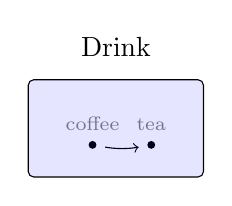
\begin{tikzpicture}
			\node[pt=coffee] at (0,1){};
			\node[pt=tea, right=1.8em of coffee] {};
			\draw[arr,->, thin] (coffee) to[bend right=10](tea);
			\node[Dom={Drink : \lab{coffee}\lab{tea}}, active] (D) {};
		\end{tikzpicture}
	\end{center}
	
	
	On the other hand, given enough time to think, you may remember you had reasons for choosing tea the last time. Some considerations might include:
	\begin{enumerate}[nosep]
		\item The coffee is not fair trade, and contributes to poor working conditions in Columbia
		\item Your previous experiences with coffee have been better than your previous experiences with tea
		\item Coffee has more caffeine than tea	
	\end{enumerate}

	Note that each of these considerations consists of two parts: another thing you assign value to (the pleasure of your previous experiences, exploited workers, caffeine), plus some belief about how a decision in one domain will impact the others (what impact does coffee have on the world, what do I remember about my experiences, what do I know about the caffeine content). We can picture this with the following diagram:
	
	\begin{center}
		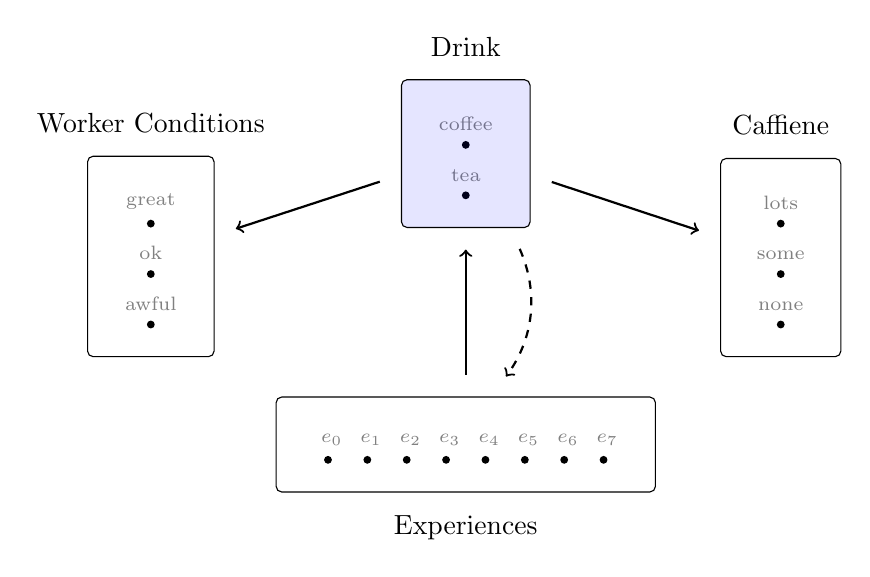
\begin{tikzpicture}
			\node[pt=coffee] at (0,1){};
			\node[pt=tea, below=1.5em of coffee] {};
			\node[Dom={Drink : \lab{coffee}\lab{tea}}, active] (D) {};
			
			
			\node[pt=lots] at (4,0){};
			\node[pt={some}, below=1.5em of lots] {};
			\node[pt={none}, below=1.5em of {some}] {};
			\node[Dom={Caffiene : \lab{lots}\lab{none}}] (C) {};
			
			\node[pt={great}] at (-4,0){};
			\node[pt={ok}, below=1.5em of great] {};
			\node[pt={awful}, below=1.5em of ok] {};
			\node[Dom={Worker Conditions : \lab{great}\lab{awful}}] (W) {};
			
			
			\foreach [evaluate=\x as \y using \x/2-1.75] \x in {0, 1, ...,7} {
%					\pgfmathmacro{\tmp}{-1 + 0.2*\x}
				\node[mpt={e\x | $e_\x$}] (e\x) at (\y,-3) {};
			}
			\node[bDom={Experiences : \lab{e0}\lab{e7}}] (E) {};
			
			\draw[arr] (D) -- (C);
			\draw[arr] (D) -- (W);
			\draw[arr, dashed] (D) to[bend left] (E);
			\draw[arr] (E) -- (D);
		\end{tikzpicture}
	\end{center}
	According to the diagram, we endorse the following decision making process: start with your ambient (prior, in analogy to Bayesian updating) preference for the decision at hand: which drink to order. Then, consider other domains you have ambient preferences attached to, the way in which this decision impacts them, and nudge your current preference in the appropriate way. While the two things on the edges look like they have some causal flavor, the one on the bottom is different: there's no way that having a drink can cause you to have one of your previous experiences. Instead, your experiences have the property of \todo{}


	Now that we have added more information to the model, let's consider what the standard modeling approach would be in this situation: we would need (1) utilities $U : \mathcal W \to \mathbb R$ over worlds, which in this case would be modeled as an assignment $\mathcal W = (D \times W \times C \times E)$ to each of the four variables (or selection of a point from each of the domains in the picture above), and also (2) a conditional probability distribution over worlds $\Pr(\mathcal W | D)$, for each choice of drink. At this point we compute expected utilities,
	
	\[  \mathop{\mathbb E} \Big(U ~\Big|~ \text{coffee}\Big) = \sum\limits_{w \in \mathcal W} U(w) \Pr(w | \mathrm{coffee}) 
	\hspace{2cm} 
 \mathop{\mathbb E} \Big(U ~\Big|~ \text{tea}\Big) = \sum\limits_{w \in \mathcal W} U(w) \Pr(w | \mathrm{tea}) \]
	
	and compare the results. Doing this computation directly has a number of draw-backs:
	\begin{itemize}[nosep]
		\item There's not a clear way of making use of partial computations: if you're halfway through your expected utility computations, you still haven't made a decision.
		\item It requires a joint distribution over all variables you care about: in our example, we would have needed to know how our experiences related to worker conditions in Columbia, how both of these relate to your caffeination levels.
		
		\item From the modeler's perspective, this whole setup changes drastically if it turns out we at the last minute remember that social signaling is relevant to the decision. Such a change causes even the collection of worlds to be different, and it's not immediately obvious if we can recycle our old utility function and probability distributions.
		
%			\item All inconsistencies have to be sorted out at all times: there are no intermediate steps where your views can be 
	\end{itemize}

%		Now, since the last time you've examined your preferences, 
	It may seem at this point like we have merely introspected a hacky algorithm which does not suffer from these issues by design, ignored the rationality guarantees provided by expected utility, and hidden the fact that the expected utility computations can often be approximated quickly with some straightforward tricks. From the classical point of view, all we needed to do was assume that $U$ is additively separable, that the independence assumptions that accord with the interpretation of the above diagram as a Bayesian Net hold, and just compute the correct answer directly. From this perspective, it looks as though our procedure is a special case of expected utility but implemented in a riskier, incremental way. 
	
	On the other hand, expected utility can be seen as a special, particularly brittle and centralized, case of our updating method, in which the only thing that matters is a special domain $\mathbb R$, there is always exactly one path that can be used to compute it, which involves integrating over all possible worlds, and we don't save any computations. In particular, by using a dashed boundary to denote a domain which does \textbf{not} accrue value, this corresponds to running our updating on the following diagram, and just computing until it converges:\\
%		Moreover, the expected utility calculations correspond to to 

	\begin{center}
		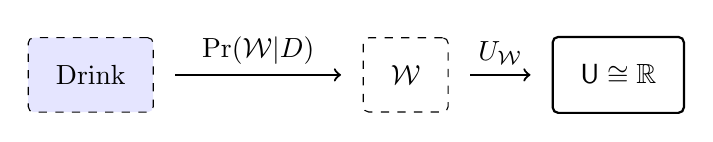
\begin{tikzpicture}
			\node[dpadded, dashed, active] (D) at (0,0) {Drink};
			\node[dpadded, dashed](W) at (4,0) {$\mathcal W$} ;
			\node[dpadded, thick](U) at (6.7,0)  {$\mathsf U \cong \mathbb R$} ;

			
			\draw[arr] (D) -- node[above]{$\Pr(\mathcal W| D)$}(W);
			\draw[arr] (W) -- node[above]{$U_{\cal W}$} (U);
		\end{tikzpicture}
	\end{center}\vspace{1em}
	
	Note also that if the preferences on $\cal W$ did not come from a utility function, but rather you simply had preferences over possible worlds, we have an even simpler picture:
	
	\begin{center}
		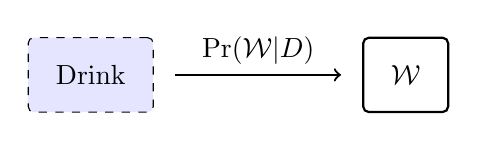
\begin{tikzpicture}
			\node[dpadded, dashed, active] (D) at (0,0) {Drink};
			\node[dpadded, thick](W) at (4,0) {$\mathcal W$} ;	
			
			\draw[arr] (D) -- node[above]{$\Pr(\mathcal W| D)$}(W);
		\end{tikzpicture}
	\end{center}\vspace{1em}
	
	This is a quick graphical illustration of why preferences representable by utility functions are a strict sub-class of preferences over worlds. Also, it suggests that a utility function is mathematically a ``belief-like'' object, tying two domains together, which is why it makes sense to define products between it and probability distributions. 

	Moreover, if the only thing we cared about was the special utility box anyway, both the additive separability and conditional independence assumptions have a graphical interpretation if we represent them in this manner. Consider the diagram below:
	\begin{center}
		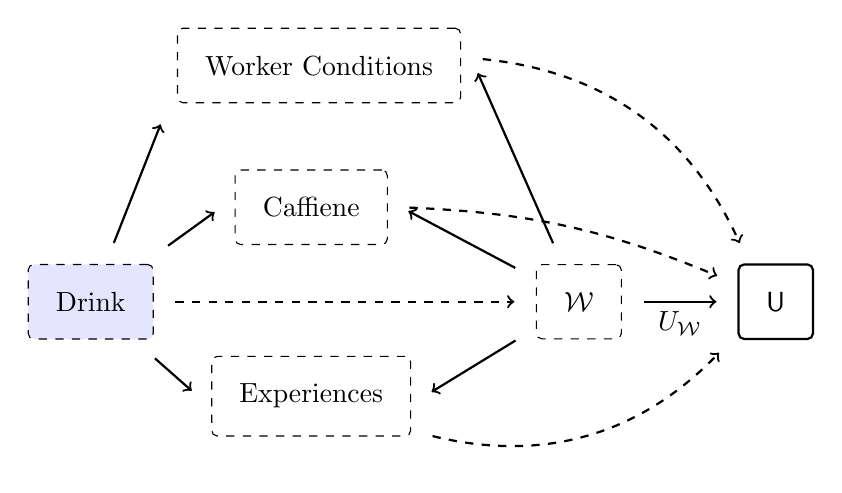
\begin{tikzpicture}
		\node[dpadded, dashed, active](D) at (1.2,0) {Drink};
		\node[dpadded, dashed](C) at (4,1.2) {Caffiene} ;
		\node[dpadded, dashed](W) at (4.1,3) {Worker Conditions} ;
		\node[dpadded, dashed](E) at (4,-1.2) {Experiences} ;
		\node[dpadded, dashed](WW) at (7.4,0) {$\mathcal W$} ;
		\node[dpadded,thick](U) at (9.9,0) {$\mathsf U $} ;
		
		
		\draw[arr] (D) -- (C.west);
		\draw[arr] (D) -- (W.south west);
		\draw[arr] (D) -- (E.west);
		\draw[arr, dashed] (D) -- (WW);
		
		\draw[arr, dashed] (W) to[bend left] (U);
		\draw[arr, dashed] (C.east) to[bend left=10] (U);
		\draw[arr, dashed] (E) to[bend right] (U);

		\draw[arr] (WW) -- node[below]{$U_{\cal W}$} (U);
		\draw[arr] (WW) -- (C.east);
		\draw[arr] (WW) -- (W.east);
		\draw[arr] (WW)  -- (E.east);
		
		\end{tikzpicture}
	\end{center}
	The line from Drink to $\mathcal W$ has to be inferred somehow, if the only way we can compute value is by going to $\sf U$ via $U_{\cal W}$. Doing this by assuming that all of the variables are independent is the only option we really have available, which fully utilizes all of the information we have in the diagram.
	
%	This is false:
%	More specifically, every triangle should commute: inferring your caffeination from the drink choice should be the same as inferring the impact of drink choice on the world, followed by a determination of your caffeination in that impact. Requiring that this hold for all three of the triangles on the left is related to the conditional independence assumption, and requiring that it hold for the three on the right is related to the additive separability one.
	
	
%	\subsubsection{Uses}
	
	The decision of what drink to have does not exist in a vacuum. Suppose you also have to decide what restaurant to go to get lunch, and also where to buy appliances, and groceries. Each of these depend on what drinks you like, among other things. This might look something like the diagram below.
	\begin{center}
		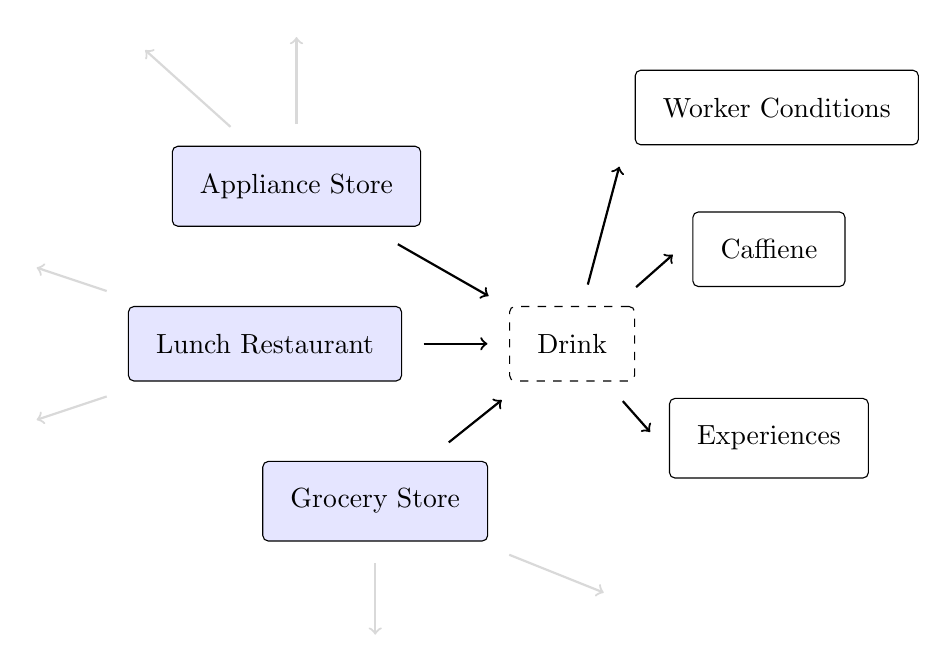
\begin{tikzpicture}
		\node[dpadded,active] (A) at (-2,2){Appliance Store};
		\node[dpadded,active] (L) at (-2.4,0){Lunch Restaurant};
		\node[dpadded,active] (G) at (-1,-2){Grocery Store};
		
		\node[dpadded, dashed] (D) at (1.5,0) {Drink};
		\node[dpadded, ](C) at (4,1.2) {Caffiene} ;
		\node[dpadded, ](W) at (4.1,3) {Worker Conditions} ;
		\node[dpadded, ](E) at (4,-1.2) {Experiences} ;
%		\node[dpadded, dashed](WW) at (6.7,0) {$\mathcal W$} ;
%		\node[dpadded,thick](U) at (9.0,0) {$\mathsf U $} ;
		
		
		\draw[arr] (D) -- (C.west);
		\draw[arr] (D) -- (W.south west);
		\draw[arr] (D) -- (E.west);
%		\draw[arr, dashed] (D) -- (WW);

		\draw[arr] (A) -- (D);
		\draw[arr] (L) -- (D);
		\draw[arr] (G) -- (D);
		
		\draw[arr, gray!30] (G) -- +(3,-1.2);
		\draw[arr, gray!30] (G) -- +(0,-1.8);
		\draw[arr, gray!30] (A) -- +(0,2);
		\draw[arr, gray!30] (A) -- +(-2,1.8);
		\draw[arr, gray!30] (L) -- +(-3,-1);
		\draw[arr, gray!30] (L) -- +(-3,1);
		
%		\draw[arr] (WW) -- node[above]{$U_{\cal W}$} (U);
%		\draw[arr] (WW) -- (C.east);
%		\draw[arr] (WW) -- (W.south east);
%		\draw[arr] (WW)  -- (E.east);
		
		\end{tikzpicture}
	\end{center}
	Having to re-compute your preference for drinks every time you have to make a decision is expensive, and while it is always possible that your drink preference would have changed in the mean time if you had re-computed it, this is probably not a very effective use of your computation, which could be spent sorting through the many other relevant features of grocery stores and restaurants. 
	
	Once again, this can be thought of in two ways: the classical one is to state that 

	\subsection{Framing Problems}
	\subsection{Heuritics: Freedom}
	
%		We can consider what would need to happen in order for this to 
					


	
	\section{Example Use Cases}
	
	
	\subsection{Serving Content}
	Since humans' preferences are not always dynamic, it is a mistake to design recommender systems as though they were. The problem of designing a recommender system is almost always framed as the task of deciding what content to display to what user at a single point in time, based on information about the content and the user, which hides potentially dynamic elements of preferences. Such a model can still accurately predict that a user's preferences have changed by looking at updated user data and considering the new user an entirely different person, but the approach of fixing this issue by trying to get more recent feature data, necessarily lags behind that source of data. While in principle it is may be possible to predict where a person's tastes are likely to go in the future, this kind of thinking mirrors only the recent past.
	
	Similarly, issues with recommender systems zeroing in on a particular niche preference set, and serving content only similar to the content the user has seen before. However, sometimes the similarity of the content is actually a detriment. For instance, if you've already watched an instructional video on integration by parts, you are less likely to click on other such videos, rather than more likely --- despite (and indeed because of) similarities between the two videos.
	
	\subsection{Framing Problems}
	It is well documented that people exhibit different preferences depending on the context and manner in which the preferences are elicited, and particularly the framing of the question. This fact is a problem for preference theories which only model world states, as they cannot distinguish between differing framings of the same logical scenario. Nonetheless, humans reliably exhibit biases dependent on the way in which a problem is framed, and perhaps reasonably so: it takes a lot of cognitive effort to see exactly what the consequences of a choice look like, language is ambiguous, and different representations of a scenario almost always highlight different salient features.
	
	\subsection{Learning Preferences from Samples}
	There is also the question of where we got our preferences in the first place. While it might be reasonable to think that a person can be born with \textit{a propensity to like video games}, it's crazy to think that people are born with actual preferences about video games. Archimedes probably did not have preferences about what video games are good, but also it would be weird if he were unable to form any.
	
	A static theory of preferences fails to provide an account of how preferences form in the first place, making them useless for understanding reasons for motivations: at the end (or if you're a logically omniscient being that economists model, at the beginning), preferences just boil down to unquestionable axioms, that could have been anything. Instead, we would like to be able to provide an account of how preferences are be formed over new concepts, implicitly providing some restrictions on the kinds of preferences it is possible to have for a given environment. By doing so, we can get a tighter bound on what agents can actually value, giving us both more predictive power, and reducing the search space for trying to infer them, in inverse reinforcement learning, content recommendation, and so forth.
	
	\subsection{Gamification}
	One particularly objectionable feature of static preference models is that they depend on 
	
	For instance, in an expected utility setting, I can say that playing a game $g$ give me 5 utils (maybe in context). Maybe I can even break this down, and say that the storyline gave me 3, while the competitive aspects are collectively responsible for 2. 
	
	But the weird feature of this is that story telling and 
	
	A particular effect that we would like to model is \textit{value capture}---
	
	\subsection{Specification of Robot Preferences}
	The problem with simply giving an agent an objective to optimize, is that people are really bad at understanding what optimizing any given objective actually means until they see it. In practice, people mis-specify objectives all the time, and are often mistakenly under the impression that they've incentivized the agent to do something slightly different. There are even numerous fairy tales and parables cautioning against this, which can be summed up with the aphorism ``be careful what you wish for''
	
	People don't have to be all that careful what they wish for around their friends and family, however, because they do not express their desires in such clear terms as objective functions, and the wishes they express are not taken literally, but rather in context with the other preferences this person has expressed, and the social context. A theory of preference dynamics would allow for both partial specification and overspecification, which may be a step towards corrigibility.
	
	\section{Some Intuition about the Framework}
	We think of preferences over most things as actually being cached computations of how to optimize other, previously held preferences, filtered through some beliefs about the world. For instance, 
	
	\begin{itemize}[nosep]
		\item A taste for ice cream can be thought of as a cached version of the evolutionary preference for staying alive, seen through the lens of food choice: perhaps a cached preference computation from times when calories were scarce.
		\item A preference for green apples over red ones might be the cached computation from the last time you were faced with a similar choice, incorporating factors such as usefulness in the kitchen, sourness, color preference, and so forth. This preference is not an intrinsic feature of your agency, but rather a cached view of other preferences through the apple lens.
		\item An affinity towards the political ideal freedom can be thought of as a cached view of your preferences over governments you've read about or experienced, seen through the lens of one particular feature: how much freedom the government offers.
		\item Vegetarianism can be thought of as a cached preference for environmentalism and reduction of animal suffering, filtered through the lens of food choice.
		\item Habits can be thought of as cached versions of your preferences (nutritional, entertainment, intellectual, structural, etc.), filtered through the lens of stimulus-response functions
	\end{itemize}
	
	With this in mind, our picture of preferences encodes a bunch of redundant information, in many different settings, and the picture is informed by the ways that the world can cause one setting to have a bearing on other related ones. 
	
	Note that it is possible to de-couple a preference from the original reasons for forming it: the first and last examples above are good illustrations. A sweet-tooth is no longer the best way to ensure evolutionary success now due to environmental distributional shift, but we retain this preference anyway. In the last example, people who became vegetarian purely for environmental and animal rights reasons, will do better on both fronts eating meat for a day in exchange for a friend abstaining for two --- and yet people are often hesitant to make this trade, because the preference acquires.
	
	If we were both cognitively unbounded and certain about what we cared about, we would not need to keep around preference domains for anything else for very long. We could just re-compute everything we needed from scratch from only our single true preference domain, which was precise enough to exactly capture the one thing we care about --- this corresponds to the classical view of static preferences.
	
	
	\subsection{Dynamics}
	The feature that drives preference changes, in this framework, is cognitive dissonance between conflicting preferences, which is why the static picture is static.
	
	%%%%%%%%%%%%%%%%%%
	There are two equivalent ways of thinking about how preference change works here: identity, and conflict.
	
	The first is by 
	
	\section{Preliminaries and Foundational Theory}
	\subsection{Preferences as Binary Relations}
	In its most basic form, a preference over a set $A$ of alternatives, i.e., the set of things we can chose between, is a binary relation $\leqc$ on $A$ that is transitive and reflexive, where $a \leqc b$ is interpreted as ``Given a choice between $a$ and $b$, I would choose $b$''. To make them self-consistent, people additionally impose axioms:
	\begin{align*}
	\forall x \in A.&~x \leqc x \tag{Reflexivity}\\
	\forall x,y,z \in A.&~(x\leqc y)~\land~( y \leqc z) \Rightarrow~(x \leqc z) \tag{Transitivity}\\
	\forall x, y \in A. &~ (x\leqc y)~\lor~( y \leqc x) \tag{Completeness}
	\end{align*}
	It is also common to speak of indifference between two alternatives ($x \sim y$), and strict preference of $y$ to $x$ ($x \prec y$), which we define as:
	\begin{align*}
		\text{Indiference:}\qquad x \sim y &~:= (x \leqc y) \land (y \leqc x)\\
		\text{Strict Preference:}\qquad x \prec y &~:= (x \leqc y) \land \lnot (y \leqc x)
	\end{align*}
%	Note that 
%	\begin{align*}
%		\forall x,y \in A.&~(x \prec y) \implies \lnot (y \prec x)\tag{Asymmetry}
%	\end{align*}
	
	\subsection{Preference Matrices}
	Because a binary relation $\leqc$ on $A$ is a function $\mat A_\leqc: A \times A \to \mathbb{B}$, taking a pair of alternatives, and returning a boolean, we can think of it as a boolean matrix indexed by values of $A$, and re-interpret the axioms above as matrix properties. This will allow us to get fuzzy preferences for continuous updates, and allow us to express things as ``the desire to make preferences more transitive'' without requiring that they always are in this state. 
	
	\begin{minipage}{0.47\linewidth}
		\begin{example}\label{ex:mat1}
			If $A = \{a_0, a_1, a_2\}$, and $A \prec B \prec C$, then using the basis $[a_0, a_1, a_2]$, we have: 
			\[\mat A_\leqc =~ \begin{matrix} & \begin{matrix}a_0 & a_1 & a_2\end{matrix} \\[0.2em]
			\begin{matrix}a_0 \\ a_1 \\ a_2\end{matrix} & \begin{bmatrix}
			1 & 1 & 1 \\
			0 & 1 & 1 \\
			0 & 0 & 1
			\end{bmatrix}\end{matrix} \]
		\end{example}
	\end{minipage}
	\hfill
	\begin{minipage}{0.47\linewidth}
		\begin{example}\label{ex:mat2}
			On the other hand, with again  $A = \{a_0, a_1, a_2\}$, if we were indifferent between all of the alternatives, we would have
			\[\mat A_\leqc =~ \begin{matrix} & \begin{matrix}a_0 & a_1 & a_2\end{matrix} \\[0.2em]
			\begin{matrix}a_0 \\ a_1 \\ a_2\end{matrix} & \begin{bmatrix}
			1 & 1 & 1 \\
			1 & 1 & 1 \\
			1 & 1 & 1
			\end{bmatrix}\end{matrix} \]
		\end{example}
	\end{minipage}\\

%	It is a theme that the entry $\mat{A}_\leqc(i,j)$ only tells half the story of the relationship between the elements $i$ and $j$; we 
	
	This representation, suggests some additional algebraic structure. The Boolean algebra $\mathbb B$ forms a semi-ring where addition is $\lor$ and multiplication is $\land$, and as a consequence, the $\mathbb B$-matrices over a finite set $A$, denoted $M_A(\mathbb B)$, also form a semi-ring, where for $\mat A, \mat B \in M_n(\mathbb B)$ we define:
	\begin{align*}
		(\mat A + \mat B)_{i,j} := \mat A_{i,j} + \mat B_{i,j} \\
		(\mat A \mat B)_{i,j} := \sum_{k \in A} \mat A_{i,k} \mat B_{k,j} 
	\end{align*}
	We can also think of the boolean algebra order-theoretically: we can define an order from addition, so that $a \leq b := (a + b = b)$, for $a, b \in \mathbb B$. Analogously, we define the matrix order on $M_A(\mathbb B)$ point-wise:
	\begin{equation*}
		(\mat A \leq \mat B) := \forall i,j \in A. ~ \mat A_{i,j} \leq \mat B_{i,j}
	\end{equation*}
	
	\begin{fact}
		If $\leqc$ is a binary relation on $A$, then $\leqc$ is complete if and only if $\mat A^T + \mat A = \mathbf 1$, where $\mathbf{1}_{i,j} = 1$
	\end{fact}

	\begin{fact}
		If $\leqc$ is a binary relation on $A$, then $\leqc$ is reflexive if and only if $\mat I \leq \mat A$, where 
		\[ \mat I_{i,j} := \begin{cases} 1 & \text{i = j}\\ 0 &\text{otherwise} \end{cases} \]
	\end{fact}
	
	\begin{prop}
		If $\leqc$ is a binary relation on $A$, then $\leqc$ is transitive if and only if $(\mat A_{\leqc})^2 \leq (\mat A_\leqc)$
	\end{prop}
	\begin{proof} 
	To make room for index subscripts, we will write $\mat A^\leqc$ instead of $\mat A_\leqc$. Unwinding the definitions:	
	\begin{align*}
		&(\mat A_\leqc)^2 \leq (\mat A_\leqc)  \\
		\iff\qquad&\forall i,j \in A.\quad  \left(\sum_{k \in A} \mat A^\leqc_{i,k} \mat A^\leqc_{k,j}\right) \leq \mat A^\leqc_{i,j}   \\
		\iff\qquad &\forall i,j \in A.\quad  \left(\sum_{k \in A} \mat A^\leqc_{i,k} \mat A^\leqc_{k,j}\right)+ \mat A^\leqc_{i,j}  = \mat A^\leqc_{i,j}\\
		\iff\qquad &\forall i,j \in A.\quad \left( (i\leqc j) \lor \bigvee_{k \in A} (i \leqc j) \land (j \leqc k) \right) \Leftrightarrow (i \leqc j)\\
	\intertext{For any  $\varphi \lor \psi \Leftrightarrow \varphi$ is equivalent to $\varphi \lor \psi \Rightarrow \varphi$, since the reverse direction always holds, which is in turn equivalent to $\psi \Rightarrow \varphi$. As a result, our expression becomes}
		\iff\qquad &\forall i,j \in A.\quad  \left(\bigvee_{k \in A} (i \leqc j) \land (j \leqc k) \right) \Rightarrow (i \leqc j) \\
		\iff\qquad &\forall i,j \in A.\quad  \lnot \left(\bigvee_{k \in A} (i \leqc j) \land (j \leqc k) \right) \lor (i \leqc j) \\
		\iff\qquad &\forall i,j \in A.\quad  \left(\bigwedge_{k \in A} \lnot\Big[ (i \leqc j) \land (j \leqc k) \Big] \right) \lor (i \leqc j) \\
		\iff\qquad &\forall i,j \in A.\quad  \bigwedge_{k \in A}\left( \lnot\Big[ (i \leqc j) \land (j \leqc k) \Big]  \lor (i \leqc j) \right) \\
		\iff\qquad &\forall i,j,k \in A.\quad   \Big[ (i \leqc j) \land (j \leqc k) \Big]  \Rightarrow (i \leqc j) \\
		\iff\qquad & \text{$\leqc$ is transitive}
	\end{align*}
	\end{proof}

	We now have a test for transitivity, that suggests that iterated products are the way to compute transitive closure. In fact, the matrix star operator from iterated application is indeed what we're looking for, but to prove this first we need a lemma:
	
	\begin{lemma}
		If $\mat A,\mat B,\mat C$ are square matrices over a (pre\footnote{a semiring that might not have identities})-semiring $(S, +, \times)$, where an ordering $\leq$ is defined from $+$ as above, and $\mat A \leq \mat B$, then $\mat A \mat C \leq \mat B \mat C$, and $\mat C \mat A \leq \mat C \mat B$.
	\end{lemma}
	\begin{proof}
		As $\mat A \leq \mat B$, which is shorthand for $\mat A + \mat B = \mat B$, we have:
		\begin{equation*}
%			\sum_{s \in S} \mat B_{i,s} \mat C_{s,j} &= \sum_{s \in S} \mat B_{i,s} \mat C_{s,j}  \\
			\mat A \mat C + \mat B \mat C = 
			\sum_{s \in S} \mat A_{i,s} \mat C_{s,j} + \sum_{s \in S} \mat B_{i,s} \mat C_{s,j}  = 
			\sum_{s \in S} (\mat A_{i,s} + \mat B_{i,s}) \mat C_{s,j} 
				= \sum_{s \in S} \mat B_{i,s} \mat C_{s,j} 
				= \mat B \mat C 
		\end{equation*}
		And therefore $\mat A \mat C \leq \mat B \mat C$. A similar proof works on the left with left distributivity. Note that we don't even need to expand the indices, as the matrices themselves form a semi-ring, so this is just weakly disguised distributivity.
	\end{proof}
	
	Now, the promised result:
	
	\begin{prop}
		If $\leqc$ is a relation on $A$, whose matrix is $\mat A$, then $\mat A^* := \mat I + \mat A + \mat A^2 + \mat A^3 + \ldots$, if it exists, is the reflexive transitive closure of $\leqc$.
	\end{prop}
	\begin{proof}
		To prove this, we must show that $\mat A^*$ is transitive, includes $\mat A$, and is included in any other reflexive transitive relation which has both of these properties. 
		As $+$ is element-wise $\lor$ in this case, if $\mat A_{i,j} = 1$, then $\mat A_{i,j}^* = \mat{I}_{i,j} \lor \mat A_{i,j} \lor \cdots = 1$, so $\mat A \subseteq \mat A^*$. The transitivity argument follows from distributivity and idempotence of $+$: 
		\begin{align*}
			\left(\sum_{n=0}^\infty \mat A^n \right)^2 &= \left(\sum_{n=0}^\infty \mat A^n \right) + \mat A \left(\sum_{n=0}^\infty \mat A^n \right) + \mat A^2 \left(\sum_{n=0}^\infty \mat A^n \right)  + \cdots \\
			&= \mat I + \mat A + (\mat A^2 + \mat A^2) + (\mat A^3 +\mat A^3 + \mat A^3) +\cdots \\
			&= \mat I + \mat A + \mat A^2 + \mat A^3 + \cdots\\
			&= \mat A^*
		\end{align*}
		This clearly works in the finite case, and can be inductively extended to countably infinite sets for boolean algebra, as $\land$ distributes even over infinite disjunctions. Finally, if $\mat A \leq \mat B$, and $\mat B$ is transitive, then we will prove by induction on $k$ that $\sum_{k=0}^n \mat A^k \leq \mat B$. First note that since $\mat B$ is transitive, we have $\mat B^2 \leq \mat B$, and so it follows inductively that $\mat B^k \leq \mat B$ for all $k \in \mathbb N$. 
		
		Now base case, for $n=0$ (i.e., $\mat I \leq \mat B$) is immediate because $B$ is assumed to be reflexive. Now suppose this holds for a particular $n$. Then,		
		\begin{equation*}
			\sum_{k=0}^{n+1} \mat A^k  = \mat A^{n+1}  + \sum_{k=0}^n \mat A^k \leq \mat B + \mat A^{n+1} \leq \mat B + \mat B^{n+1} = \mat B (\mat I + \mat B^n) \leq \mat B (\mat I \mat B) = \mat B^2 \leq \mat B
		\end{equation*}
		Passing to the limit, we therefore have $\mat A^* \leq B$, as desired.		
	\end{proof}
	\begin{remark}
		Because 1 is an anihilator for $\lor$, closures always exist (if $A$ is finite) for $M_A(\mathbb B)$ \cite{pathproblems-lec3}, making it a Kleene Algebra.
	\end{remark}
	\begin{remark}
		We can also think of a preference domain $(A,~\mat A\colon A\times A \to S)$ over a semiring $S$ as an $S$-enriched category. In particular, orders are thin categories. As we will see, the links can be thought of as profunctors on these categories, and many categorical constructions have useful analogs.
	\end{remark}

	\subsubsection{Interpretations}
	Relaxations of this theory to fuzzy semirings, combined with information from other domains, will be the formal basis of our preference updating theory. As sanity checks, we can now go through some other common interpretations of semiring matrices, particularly over boolean algebras, and verify that the preference interpretation makes sense:
	
	\begin{enumerate}[nosep]
		\item If we think of a set of propositions $S$ as a preference domain, where we prefer ``truer'' statements, i.e., $s \leqc t$ if $s \Rightarrow t \in S$, then $(\mat S_\leqc^*)$ is the inferred preference on 
	\end{enumerate}

	\subsection{Non-Boolean Preference Matrices}
	One reason to react against purely order-based preference models is that they throw away a lot of important information. For instance, perhaps prefer vanilla ice cream to chocolate, and chocolate ice cream to 47 years in prison. One of these choices is a lot easier than the other. Moreover, this is not purely an internal feeling: putting on our frequentist hats for a moment, repeated exposure to this choice, would likely result in some probability mass on selections of both vanilla and chocolate ice cream, but no takers for the prison.
	
	This is one of many benefits utility has over preference orderings. Recall that a utility function on a set of alternatives $A$ is a function $u : A \to \mathbb R$, the value of which one tries to maximize with choices. 
	However, assigning utilities to things is generally considered less general (despite the above concern) than the order-theoretic approach, because not all valid preferences can be described using utility functions: for this to be the case, preferences must be both transitive and complete. In the presence of uncertainty (i.e., choices take the form of acts: maps from states to outcomes), Savage \cite{savage1972foundations} shows that a number of additional restrictions are necessary to represent a preference order with a probability distribution over states and a utility function on outcomes. 
	
	With real-valued preference matrices, we can get the representational flexibility of both approaches: any preference relation $\leqc$ on a set $A$ can be represented just as we did in examples \ref{ex:mat1} and \ref{ex:mat2}, by setting
	\[ \mat A^\leqc_{i,j} := \begin{cases} 1 & \text{if $i \leqc j$} \\ 0 & \text{otherwise}\end{cases}\]
	On the other hand, we can also represent a utility function $u : A \to \mathbb R$, as a matrix, in several useful ways:
	\begin{align*}
		\big[\mat A^{+ u}\big]_{i,j} &:=   u(j) - u(i) 	\\[0.3em]
		\big[\mat A^{\times u}\big]_{i,j} &:= \big[\exp \mat A^{+u}\big]_{i,j} = \exp ( u(j) - u(i) ) \\[0.3em]
		\big[\mat A^{\sim u}\big]_{i,j} &:= \left[\frac{1}{\mat 1 + \exp(- \mat A^{+ u})}\right]_{i,j} = \frac{1}{1+\exp ( u(i) - u(j) )}
	\end{align*}

	The different representations will allow us to deal with utilities as matrix factorizations, by representing combinations multiplicatively rather than aditively, as in proposition \ref{prop:decomp}, and allow us to make use of existing theory in \cite{elsner2004max}. But first, some more basic, sanity results. We would like the different embeddings to generate the same orders:

	\begin{prop}
		If $X$ is a set, and $\leqc$ is an order, corresponding to according to a utility function $u : X \to \mathbb R$, i.e., $x \leqc y \Leftrightarrow u(x) \leq u(y)$, then 
		\[
			\mat X^\leqc = H(\mat X^{+u} ) 
	 		 = H(\mat X^{\times u} - \mat 1)
	 		 = H(\mat X^{\sim u} - \tfrac{1}{2}\mat 1)
		\]
		where $H$ is the right-biased pointwise heaviside function, 
		\[H(\mat T)_{i,j} := \indi{\mat T_{i,j} \geq 0} = \begin{cases} 0 & \text{if}~\mat T_{i,j} < 0 \\ 1 & \text{if}~\mat T_{i,j} \geq 0\end{cases}\]
	\end{prop}
	\begin{proof} Each can easily be reduced to $\mat X^\leqc$, as each of $\mat X^{+u}$, $\mat X^{\times u}$, and $\mat X^{\sim u}$ are all strictly monotonic functions of the difference in utility at each coordinate:
		\begin{equation*}
			H(\mat X^{+u} )_{i,j} = \indi{\mat X^{+u}_{i,j} \geq 0} = \indi{u(j) - u(i) \geq 0} = \indi{u(j) \geq u(i)} = \indi{i \leqc j} = \mat X^\leqc 
		\end{equation*}
		\begin{equation*}
			H(\mat X^{\times u} - \mat 1)_{i,j} = \indi{\mat X^{\times u}_{i,j} \geq 1} = \indi{\exp(u(j) - u(i)) \geq 1} = \indi{u(j) \geq u(i)} = \indi{i \leqc j} = \mat X^\leqc 
		\end{equation*}
		\begin{equation*}
		H(\mat X^{\sim u} -\tfrac{1}{2} \mat 1)_{i,j} = \indi{ \mat X^{\sim u}_{i,j} \geq \tfrac{1}{2}} = \indi{\dfrac{1}{1 + e^{u_i - u_j}} \geq \tfrac{1}{2}} 	
			= \indi{1 + e^{u_i - u_j} \leq 2}= \indi{e^{u_i - u_j} \leq 1} = \indi{u_i \leq u_j} = \indi{i \leqc j} = \mat X^\leqc 
		\end{equation*}
	\end{proof}

	In the case of $\mat X^{\sim u}$, we have a much stronger limit coherence result, which does not require rounding or shifting:
	\begin{prop} For any set $X$ with utility $u : X \to \mathbb R$, whose induced ordering on $X$ is $\leqc$, we have
		\[ \lim\limits_{t \to \infty} \mat X^{\sim t u} = \mat X^\leqc, \]
	where $tu := x \mapsto t\cdot u(x)$ is a scaled version of $u$, and therefore induces the same ordering.
	\end{prop}

	\begin{prop}\label{prop:decomp}
		A non-negative preference matrix $\mat A : X \times X \to \mathbb R_{\geq 0}$ is a rank-1 matrix with $\mat A \odot \mat A^T = \mat 1$ (where $\odot$ is the element-wise, or Hammard product), if and only if $\mat A$ is multiplicatively representable by a utility function, i.e., there exits $u : X \to \bar{\mathbb  R}$ such that $\mat A = \mat X^{\times u}$
	\end{prop}
	\begin{proof}
		We'll start with the easier, backwards direction. If $\mat A = \mat X^{\times u}$, then
		\[ \mat A_{i,j} = \big[\mat X^{\times u}\big]_{i,j} =  \exp(u(j) - u(i)) = \left(e^{u(j)}\right)\left(e^{-u(i)}\right) \]
		Therefore we can write $\mat A =  x^T  y$, where $x$ and $y$ are $\mathbb R$-vectors over $X$, defined as $ x_i = e^{-u(i)}$ and $ y_j = e^{u(j)}$, so $\mat A$ is rank-1. Also, we have 
		\[ \big[\mat A \odot \mat A^T\big]_{i,j} =  \mat A_{i,j} \mat A_{j,i} = \frac{e^{u_j}}{e^{u_i}} \frac{e^{u_i}}{e^{u_j}} = 1\]
		
		On the other hand, now suppose that $\mat A$ is rank-1, with $\mat A \odot \mat A^T = \mat 1$. Because it is rank-1, there exist real valued vectors $x$ and $y$ over $X$ such that $\mat A  = x^T y$, and so the second condition becomes: $x^T y \odot y^T x = \mat 1$, or equivalently,
		\[ \forall i,j \in X.\quad x_i y_j y_i x_j  = 1 \qquad\implies\qquad x_j y_i = \frac{1}{y_j x_i} \]
		We now define $u(k) := \frac{1}{2} (\log y_k - \log x_k) = \log\sqrt{y_k / x_k}$, so that
		\[ \big[\mat X^{\times u}\big]_{i,j} = \exp\left(\log\left(\sqrt{y_j/x_j}\right)- \log\left(\sqrt{y_i/x_i}\right)\right) 
			= \exp\log\sqrt\frac{y_j x_i}{x_j y_i} 
			= \sqrt{(y_j x_i)(y_j x_i)} = x_i y_j = \mat A_{i,j}\]
	\end{proof}

	

	\begin{coro}
		A preference matrix $\mat A : X \times X \to \mathbb R$ is additively representable by a utility function (i.e., $\exists u : X \to \mathbb R$ such that $\mat A = \mat X^{+u})$ if and only if $\mat A$ is skew symmetric and $\exp (\mat A)$ is rank-1.
	\end{coro}
	
	
	
	\subsubsection{Non-standard Semi-rings and Low-Rank Decompositions}
	\textbf{Peron-Frobenius Vector.}
	
	\textbf{Subtropical-Eigenvector.} \cite{elsner2004max}\cite{elsner2010max}
	
	\subsubsection{Parameterized Weights}
	
	\subsection{Domain Links}
	Preference domains are only half of the picture: we also want to link them together, and describe how preferences in one domain can impact ones in other domains. To do this, we will need some mathematical formalism to describe them. For now\footnote{For example, I get the sense we could also have used joint probabilities and undirected models to get a Markov Network, or even a causal model, where the structural equations are edges, and the nodes are variables. However, this would require different notions than the ones described here.}, we will formalize these as conditional probability distributions. A link $L$ from one preference domain to another is just a function 
	\[ L : A \to \Delta B \]
	which yields a probability distribution $\Delta B$ on $B$ for every element of $A$. This is thought of as the impact of the choice of alternatives in domain $A$ on the domain $B$. If both $A$ and $B$ are discrete, these conditional distributions can be represented as stochastic matrices\footnote{If the edges were undirected and we had started with a Markov random field, these would be matrices of the same shape, representing joint probability distributions} (matrices $\mat L : A \times B \to [0,1]$ such that $\forall a \in A. \sum_{b \in B} \mat L_{a, b} = 1$); for continuous domains, we can represent them as Markov kernels, which have analogous properties for the more complicated setting of measurable spaces.
	
	\subsection{Dynamics}
	In addition to keeping track of preferences, the whole point is to provide a prescription for how they should change over time. There are several driving forces we could consider: we have already vaguely suggested iterative matrix powers and low-rank approximation as methods of compressing data and pushing towards transitivity (it would take only a single matrix factorization to find a loss-minimizing solution), and it's straightforward to use these results to create differential pressure for complete, reflexive, and anti-symmetric preferences. 
	
	All of these are relatively well-known results, and apply only to a single domain; for us, the driving force will come from the interaction between them. In fact, this updating method is strictly more general:

	\begin{conj}
		If $(D, \leqc)$ is a preference domain, and a model 
		\[ \mathcal D = \Big\{ \{d, d', \bullet\}, \leqc\Big|_{d,d'} \Big\}_{d \neq d' \in D},\qquad
			\mathcal B(i,j) = \begin{cases}
				
			\end{cases}
			\] 
	\end{conj}
	
	As a first pass, note that if we had a degenerate distribution (a function) $f : X \to Y$, and we had preferences on $Y$ but not $X$, we could define $x_1 \leqc_X x_2 := f(x_1) \leqc_Y f(x_2)$. It is an important feature that this process of building up preferences backwards, in the reverse direction of the links, is the natural way to form them. In fact, to go the other direction, you need to apply Bayes' rule or compute a pseudo-inverse to get something that can be used the link going the other way. 
	
	\begin{example}
		If the preferences on $Y$ are represented by utilities $u : Y \to \mathbb R$, then the preferences on $X$ induced by a functionX $f$ and $Y$ are given by $u \circ f$. 
		
		\begin{center}
			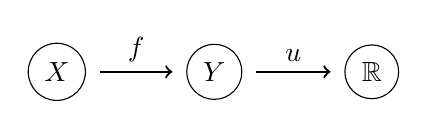
\begin{tikzpicture}
			\node[draw, circle] (X) at (0,0){$X$};
			\node[draw, circle] (Y) at (2,0){$Y$};
			\node[draw, circle] (U) at (4,0){$\mathbb R$};
			
			\draw[->, thick, shorten <=5pt, shorten >=5pt] (Y) -- node[above]{$u$} (U);
			\draw[->, thick, shorten <=5pt, shorten >=5pt] (X) -- node[above]{$f$} (Y);
			\end{tikzpicture}
		\end{center}
		
		If we only had a function $Y \to X$, and not one from $X \to Y$, then there would be no natural composition of the parts at our disposal to form a utility function on $X$.
	\end{example}
	
	\begin{example}
		We can think of
	\end{example}\vspace{1.5em}	


	\begin{prop}
		If $A, B$ are preference domains, $\mat B = \mat B^{+u}$ is additively represented by $u$, and $\mat P : A \to \Delta B$ is a stochastic matrix, then the preferences $\mat A := \mat P \mat B \mat P^T$ suggested by $\mat B$ filtered through $\mat P$ is represented by expected utility $\mathbb E u$.
	\end{prop}
	\begin{proof}
		\begin{align*}
			\mat A_{il} &= \sum_{j,k \in B} \mat P_{i,j} \mat B_{j,k} \mat P_{l,k} \\
				&= \sum_{j,k \in B} \mat P_{i,j}  \mat P_{l,k} (u_k - u_j) \\
				&= \sum_{j \in B} \mat P_{i,j} \left[ ~\sum_{k \in B} \mat P_{l,k} (u_k - u_j)\right]\\
				&= \sum_{j \in B} \mat P_{i,j} \left[ ~\sum_{k \in B} \mat P_{l,k} u_k - \sum_{k \in B} \mat P_{l,k} u_j \right] \\
				&= \sum_{j \in B} \mat P_{i,j} \underbrace{\left[ ~\sum_{k \in B} \mat P_{l,k} u_k  \right]}_{\text{indep. of $j$}} -  \sum_{j \in B} \mat P_{i,j} u_j \underbrace{\sum_{k \in B} \mat P_{l,k}}_{\text{column sums to 1}} \\
				&= \left[ ~\sum_{k \in B} \mat P_{l,k} u_k  \right] \underbrace{\sum_{j \in B} \mat P_{i,j}}_{\text{column sums to 1}} -  \sum_{j \in B} \mat P_{i,j} u_j \\
				&= \left[ ~\sum_{k \in B} \mat P_{l,k} u_k  \right]  -  \sum_{k \in B} \mat P_{i,k} u_k \\
				&= \mathop{\mathbb E}\limits_{k \sim P(l)} u(k) - \mathop{\mathbb E}\limits_{k \sim P(i)} u(k)
		\end{align*}
	\end{proof}

	\section{Present Formalism}
	\subsection{Representation}
	At each point in time, a representation of the agent's state $(\mathcal D_t, \mathcal B_t)$ consists of a collection of preference domains $\mathcal D_t = \{ (D, \mat D) \}$, as well as a collection of links $\mathcal B_t$ between connecting some subset of pairs of domains together,	
	
	\[  \mathcal B_t \subseteq \prod_{A, B \in \mathcal D_t} \Big( A \to \Delta B \Big) \] 
	
	i.e., for some subset of pairs of domains $\{ (A_i, B_i) \}_i$, we have a probability distribution $\Delta B_i$ over $B_i$ associated each element of $A_i$. We will write $B [X \to Y]$ or $\Pr(Y | X)$ to denote the conditional distribution $B \in \mathcal B$ over $Y$ whose co-domain is $X$.
	
	
	\begin{remark}
		Fixing a time $t$, if we were to forget the orderings and treat the domains as sets, and the edges formed by $\mathcal B_t$ are acyclic, then $(\mathcal D_t, \mathcal B_t)$ forms a Bayesian Network.
	\end{remark}
 
 	
 	
 	\subsection{Dynamics}
	
	
	
	For each link, whose conditional distribution we imagine being parameterized by some latent variables $\theta$, we define the inconsistency at a domain $D$ as the sum of differences between 
	\[ \zeta_\Theta(D) = \left\lVert \sum_{B[D \to X]} B^T \mat X B - \mat D \right\rVert_F \]
	where $\Theta$ contains the parameters required to generate each of these: the link $B$, and the preferences $\mat X$ and $\mat D$.
 	\footnote{In the previous version, we defined the consistency of a link $B : X \to \Delta Y$ as 
 	 	\[ \zeta\big(B[X \to Y]\big) =  \sigma \left( \left(1- \frac{|W_X - W_Y|}{W_X + W_Y}\right) \sum_{x,x' \in X}\sum_{y,y' \in Y} X(x,x') Y(y,y') B(x)(y) B(x')(y') \right) \]
 	% 	where $\sigma : \mathbb R \to [-1, 1]$ is an activation function such as sigmoid or $\tanh$, $B(y)(x)$ is the probability mass on $y$ in the distribution $B(x)$, and for a domain $D$, $D(d, d')$ is a signed preference indicator, defined as 
 		where 
 	 	$ D(d, d') := \begin{cases}
 	 		1 & d \prec_D d' \\
 	 		-1 & d \succ_D d' \\
 	 		0 & \text{otherwise}
 	 	\end{cases} $.  \todo{Show relationship}}	
 	We can also sum across the entire graph to get a measure for the whole model:
 	\[ \zeta(\mathcal D, \mathcal B) = \sum_{D \in \mathcal D} \zeta_\Theta(D) \]
 	
 	The update rule is now just gradient descent on the parameters $\Theta$ with respect to the global inconsistency:
 	
 	\[ \frac{\partial \Theta}{\partial t} = - \eta \nabla_\Theta \sum_{D \in \mathcal D} \zeta_\Theta(D) \]
 	
 	
 	\begin{remark}
 		If $\mathcal D$ consists of only a dingle domain $D$, with the identity distribution $\mathcal B = {B(x,y) = \delta_{x,y}: D \to D}$, then $\mathcal D$ is consistent, i.e., $\zeta(\mathcal D, \mathcal B) = 0$. Similarly, if there are no links, (or only identity links), then the model is consistent, because in each case the sum is vacuously zero. 
 	\end{remark}
 	
% 	Finally, the update rule is just backpropagation of the consistency through the parameters: for each parameter 
% 	\[ p \in \bigcup_{B[X\to Y] \in \mathcal B}  \Bigg( \{ X(x,x') | x, x' \in X\} \cup \{ Y(y, y') | y,y' \in Y\} \cup \{ W_X, W_y \} \cup \{B(x)(y) | x \in X, y \in Y\}  \Bigg) \]

%	\[ \frac{\partial \zeta(B) }{\partial B(x)(y) } \]
	
		
	\section{Revisited Examples}
%	Now that we have some formalism,
	
	\subsection{Framing Problems}
%	Suppose there are two framings of a decision problem, one between the alternatives $X$ and the other between the alternatives $Y$. At first, suppose you do not know how $X$ and $Y$ relate to each other, but are instead separately given hypothetical scenarios in which you are asked to choose in both cases. You decide that:	
%	\[ x \prec x' \qquad\text{and}\qquad y \succ y' \]
%	You are reasonably confident about both of these decision, but you have more confidence in your preference on $X$, because you've had to make the choice in this context before $(W_X = 0.95, W_Y=0.8)$. Upon looking at the situation more closely, however, you discover that there is actually a logical equivalence between $x$ and $y$, and between $x'$ and $y'$ (denote this bijection $f : X\to Y$). Your preferences are now in conflict, and we calculate
%	\begin{align*}
%		\zeta(f) &= \sigma \left( \left(1- \frac{0.15}{1.75}\right) \sum_{a,a' \in X}\sum_{b,b' \in Y} X(a,a') Y(b,b') B(a)(b) B(a')(b') \right) \\
%		&= \sigma \left( 0.914 \sum_{a,a' \in X} X(a,a') Y(f(a), f(a'))  \right) \\
%		&= \sigma~ \bigg( 0.914 \Big(  X(x,x') Y(f(x), f(x')) + X(x',x) Y(f(x'), f(x))  \Big) \bigg) \\
%		&= \sigma~ \bigg( 0.914 \Big(  1 \cdot Y(y, y') + (-1) \cdot Y(y', y)  \Big) \bigg) \\
%		&= \sigma (-1.83)
%	\end{align*}
	
	
	\subsection{Learning from Samples}	
	\subsection{Serving Content}
	
	In this simple example, we will consider 5 domains: Song Instances ($I$), 
	
	\subsection{Gamification}
	\subsection{Specification of Robot Preferences}
	
%	\section{Plausible Theoretical Results to Chase}
%	
%	\begin{itemize}
%		\item If we fix a maximum representation size (number of bits, comparisons, or the like), then the optimal strategy (relative to the ``true'' experience domain, which we cannot represent forever) in terms of preference fidelity is to utilize a large number of domains, rather than just a few big ones. Reasons: combinatorial explosion of orderings for big sets; generalization to unseen examples.
%		
%	\end{itemize}
	
	\section{Relation to Other Models}
			
	\subsection{CP Net Problems}
	The CP semantics are in many ways appealing: the dominance of $a$ over $\bar a$ independent of context seems to be a really nice way of capturing the utility brought by $a$ independent of the context of everything else. However, CP Nets are not well-behaved under changes of perspective, and lead to strange results if you think in terms of expected utility. The primary issue is that all of the variables are assumed to be independent, so that the space $\cal W$ of possible worlds is just the product of all of the individual variables:
	
	\[ \mathcal W \cong \prod_{X: \mathcal X} \Omega_X \] 
	
	Depending on how you think about it, there's always an injection one direction--- a world results in a setting of all of the variables:
	\[ \mathcal W \to \prod_{X: \mathcal X} \Omega_X \] 
	but even this may not be in keeping with the way we might want to use these models: some variables might not be relevant or well-defined in all contexts. For instance, people use choice of food as an example variable all the time: the variable represents my selection of dinner at restaurant $X$. But such a variable does not mean anything if I decide not to eat, or if I go to restaurant $Y$ which serves different items. One way to fix this might be to add a special ``not applicable'' value in the range of each variable like this, but now we've exacerbated our first problem even further: what does the world where ALL variables are set to ``not applicable'' look like? This failure to have a natural correspondence causes a number of problems:
	
	\subsubsection{Incompatibility with Expected Utility}
	
	Suppose that I'm choosing from 
	
	\subsubsection{Causes problems for Logical and Causal Structure}
	
	\printbibliography
	
\end{document}